\documentclass[11pt,a4paper]{article}
\usepackage[T1]{fontenc}
\usepackage{amssymb,amsmath}
\usepackage{txfonts}
\usepackage{microtype}

\usepackage[a4paper, total={6in, 10in}]{geometry}

% For figures
\usepackage{graphicx}
\usepackage{subfigure} 

% For citations
\usepackage{natbib}
\usepackage{hyperref}
\usepackage{url}
\urlstyle{same}
\bibliographystyle{icml2017}
\newcommand{\ubar}[1]{\text{\b{$#1$}}}

\renewenvironment{abstract}
   {
\centerline{\large\bf Abstract}
    \vspace{-0.1in}\begin{quote}}
       {\par\end{quote}\vskip 0.1in}

\begin{document}
\twocolumn[
\title{Natural Computing 2019/2020: Assignment \\ Genetic programming}
\author{School of Informatics, University of Edinburgh \\ s1653529}
\maketitle
]

\begin{abstract} 
\small
With Charles Darwin's publication of The Origin of Species he introduced the basis of a theory that would only gain in influence and importance up until the present time \citep{Darwin}. With the emerging concepts of various algorithms it also found its place in the field of Computer Science, more specifically, it unfolded into the field of Genetic Programming.
This paper puts forward multiple approaches on how genetic programming can be used to generate polynomials that produce as many prime numbers as possible from a given input.
It continues with the presentation of different integer functions for said purpose and finishes with an outlook on alternative applications of genetic algorithms such as neural networks. 
\end{abstract} 
\section*{Introduction}
A number $p$ is a Lucky number of Euler if and only if the prime-generating polynomial $n^2-n+p$ is prime for $n=1, 2, ..., p-1$. It has already been mathematically proven that the only lucky numbers are 2, 3, 5, 11, 17, and 41 \citep{Euler}. This paper does not try to disprove Heegner and Stark \citep{Euler} through extensive exploration as this would be a waste of energy and time. This paper attempts to explore various polynomials, later more general function-combinations and their ability to produce primes.
\\ \\
Genetic Programming starts out with a population of computer programs. These programs can be chosen at random, initialised by another algorithm or initialised according to a specific distribution. It then proceeds to evaluate all programs in the population. The program evaluations are done through a so called fitness function. Subsequently, the most useful programs are kept from the population while the less useful programs are discarded. This step will be referred to as the selection process. From this reduced population, a subset is selected with the aim to recombine the programs within and replenish the reduced population by a certain amount. This process is denoted as the crossover phase. It then continues to iteratively apply these last two steps to the population until the predefined terminal condition is met.
\\ \\
This paper starts out with an attempt to reproduce the polynomial $x^2+x+41$ with a Genetic Algorithm. The results will serve as a baseline model. Since it is a lot faster than the GP-algorithm it will help to establish reasonable bounds for our parameters. The parameters are chosen is such a way that they are comparable. The GA offers a sensible starting point. Followed by that, it will present an implementation of a Genetic Program and the experiments that were carried out with it. Lastly, it will combine the GP and Simulated Annealing to reduce the number of initially useless programs and offers an outlook on the applications of GPs.
\section*{Basic Concept}
\subsection*{Fitness function}
For the evaluation of the GA and the GP a function $f$ is utilized that combines three fitness functions by adding their scores. The scores are not weighted. The first fitness function returns the number of primes that were produced by the polynomial on a given input interval. The second fitness function returns the maximal number of consecutively produced primes on the given input interval $X = [0, 200)$. The last fitness function only returns the number of primes that are consecutively produced when starting at the lower bound of the input interval. A polynomial $p$ is evaluated via
\begin{align*}
f(p) = &f_1(p)+f_2(p)+f_3(p) \\
f_1(p) = &|\{p(x_i) \in \mathbb{P} \; | \; x_i \in X \}| \\
f_2(p) = &\max_{x_k \in X}|\{x_{i} \; | \; x_{i}, x_{i-1}, ..., x_k \in X, \\ & p(x_{i}), p(x_{i-1}), ..., p(x_k) \in \mathbb{P} \}| \\
f_3(p) = &|\{x_{i} \; | \; x_{i}, x_{i-1}, ..., x_0 \in X, \\ & p(x_{i}), p(x_{i-1}), ..., p(x_0) \in \mathbb{P} \}|,
\end{align*}
where $\mathbb{P}$ denotes the set of prime numbers.
\subsection*{Populations}
The GA/GP starts with a population of polynomials of a given size. Multiple populations can be chosen to evolve in parallel. The populations merge whenever a critical, predefined population size is reached. The GA/GP iteratively goes through the selection process followed by the repleshing of the population. The GA/GP stops and returns its result as soon as the population size stagnates.
\subsection*{Selection}
In the selection process the polynomials with a fitness score above the population's fitness mean $f_{\mu}$ remain in the population. The rest of the population is discarded. The selection process redefines a population $P_r$ via
\begin{align*}
P_r \leftarrow \{p \in P_r \; | \; f(p) \geq f_{\mu}\}
\end{align*}
\subsection*{Replenishment}
Subsequently, the number of the discarded polynomials $P_d$ is determined. The remaining polynomials $P_r$ are then taken and recombined in the crossover phase. The population is replenished by an amount $\eta \cdot |P_d|$ where $\eta$ is the replenishing-rate also denoted as the birth-rate here. We summarize the replenshing phase via
\begin{align*}
P_r = P_r \cup \; Crossover \left(\bigcup_{i=1}^{\eta \cdot |P_d|} p_i, \bigcup_{j=1}^{\eta \cdot |P_d|} p_j\right), \\ \; p_i, p_j \sim D(\epsilon),
\end{align*}
where $\epsilon \propto 0.1 \cdot |P_r|$ and avoids zero-divisions. The crossover-function recombines features of the polynomials from the two given input sets. This will be explained in later sections. $D(\epsilon)$ is a probability distribution over $P_r$ following 
\[ 
d(p|\epsilon)= \frac{f(p)+\epsilon}{\sum_{p_k \in P_r} (f(p_k) + \epsilon}.
\]
\section*{Baseline}
As mentioned before, a GA was chosen to represent our baseline for comparisons. \\
The chromosome of a polynomial in the implemented GA consists of its coefficients. The bound for the coefficients is predefined. The bound of the order of the polynomial is also set beforehand and can be regarded as an additional feature in the polynomial's chromosome. The coefficients and the order are initialised via a uniform distribution over the given bounds. Firstly, the order is determined. The coefficients follow. \\
The {\bf crossover-function} takes one polynomial from the first input set and combines it with another polynomial of the second input set with a coinciding index. Hence, each pair produces one offspring polynomial. It is very much possible that a polynomial is recombined with a copy of itself. \\
The recombination works through extending both coefficient arrays with zeros to a length that goes up to the order constraint. The new polynomial is then formed by selecting either of the respective coefficients from the two arrays factor-wise. \\
The resulting array is then passed through mutation function with a with a predefined mutation probability. The mutation function then selects a coefficient from the zero-extended resulting array and substitutes it by a new coefficient value selected from the uniform distribution over the coefficient bounds. The leading zeros are then discarded. \\ \\
For $x^2+x+41$ we record a fitness score of 236, producing 156 primes on the input interval. Evidently, the starting streak is the longest streak with a length of 40 consecutively produced primes. After several trials the GA that reproduced the polynomial in a reliable manner had one population of 5000 polynomials, a birth-rate of 0.7, a mutation-rate of 0.1, a coefficient bounding of $[1, 41]$, and an order restriction of at most degree 2. It converged after just under 30 generations.
\begin{figure}[h]
\centering
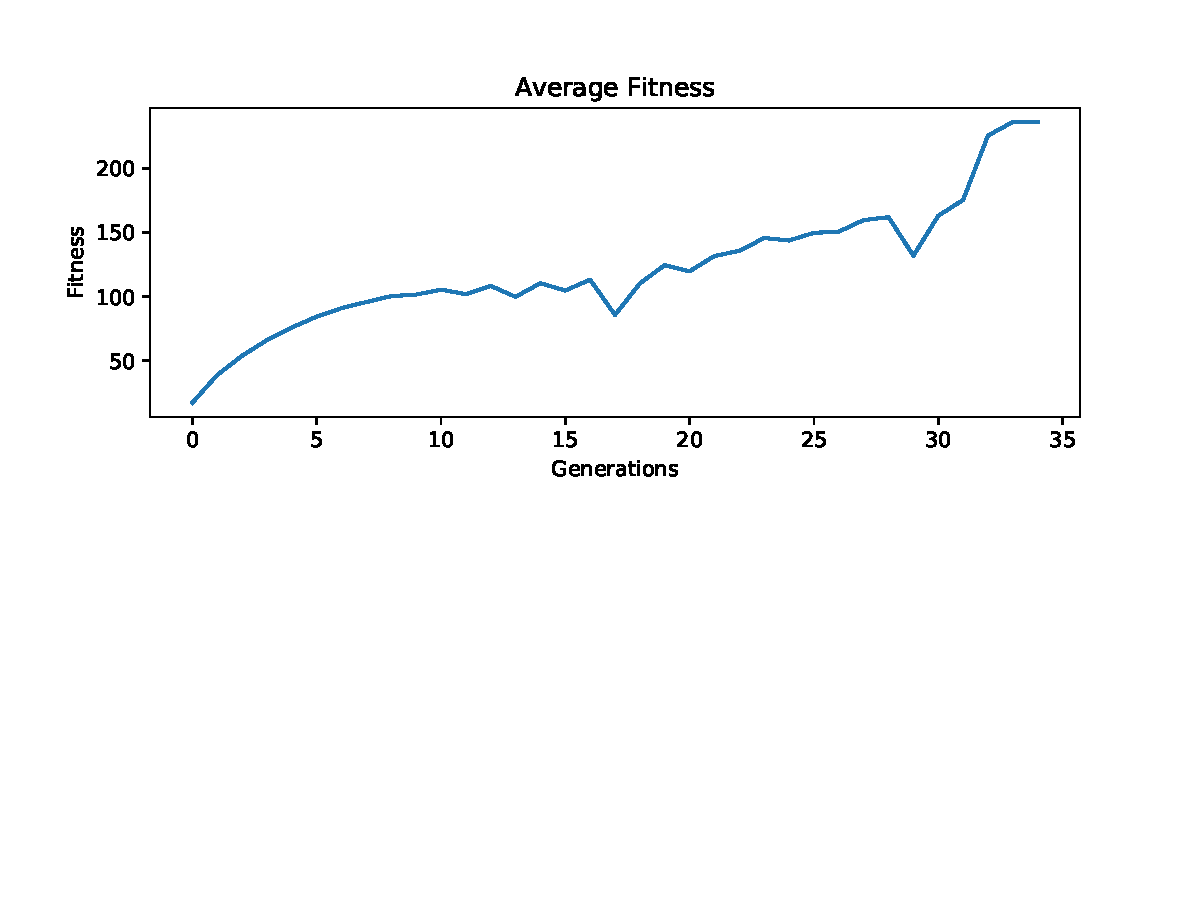
\includegraphics[scale=0.41, clip, trim=0.5cm 7cm 0.5cm 0.1cm]{../../NatComputingCW/reproduction_ga.pdf} 
\end{figure}
\subsection*{Experiments}
\section*{GP-Implementation}
\subsection*{Concept}
\subsection*{Experiments}
\subsection*{Algorithm variations}
\subsection*{Concept}
\subsection*{Experiments}
\section*{Outlook}
\bibliography{example-refs}

\section*{Appendix}

\end{document}